
%(BEGIN_QUESTION)
% Copyright 2007, Tony R. Kuphaldt, released under the Creative Commons Attribution License (v 1.0)
% This means you may do almost anything with this work of mine, so long as you give me proper credit

Imagine a situation where two different conductivity probes are immersed in the same container of water.  One probe is toroidal, while the other is a 4-electrode ``contact'' style: 

$$\includegraphics[width=15.5cm]{i03073x01.eps}$$

In both cases, the excitation signal (Ext.) is alternating current (an AC voltage source for the toroidal probe and an AC current source for the contact probe).  In both cases, the probe has a pair of wires outputting the ``Sense'' signal (normally going to an electronic amplifying circuit for conditioning and conversion into a 4-20 mA DC instrument signal).

As table salt (NaCl) is added to the water, one probe's ``sense'' signal will grow stronger while the other probe's ``sense'' signal will diminish.  Identify which is which, and explain why in each case.

\underbar{file i03073}
%(END_QUESTION)





%(BEGIN_ANSWER)

With increasing conductivity, the toroidal probe generates an increasing AC current circulating through the salty water.  This increased electric current through the water passes through the center of both toroidal coils, inducing a stronger voltage in the sensing coil.

\vskip 10pt

With increasing conductivity, the water becomes less resistive.  This results in less voltage drop between the sensing electrodes for any given amount of current between the excitation electrodes.


%(END_ANSWER)





%(BEGIN_NOTES)

%INDEX% Measurement, analytical: conductivity

%(END_NOTES)


